\documentclass[../../main/main.tex]{subfiles}
\graphicspath{{./figures/}}

\dominitoc
\faketableofcontents

\renewcommand{\mtcSfont}{\small\bfseries}
\renewcommand{\mtcSSfont}{\footnotesize}
\mtcsettitle{minitoc}{}
\mtcsetrules{*}{off}

\makeatletter
\renewcommand{\@chapapp}{Induction -- chapitre}
\makeatother

% \toggletrue{student}
% \toggletrue{corrige}
% \renewcommand{\mycol}{black}
% \renewcommand{\mycol}{gray}

\hfuzz=5.003pt

\begin{document}
\setcounter{chapter}{1}

\settype{book}
\settype{prof}
\settype{stud}

\chapter{Actions mécaniques du champ magnétique}
\label{ch:ind_meca}
\epigraph{\openquote\textit{%
		Sire, je n’avais pas besoin de cette hypothèse.
	}%
	\closequote}{Pierre-Simon \textsc{Laplace} à \textsc{Napoléon}, \textit{circa} 1800}

\vspace*{\fill}

\begin{tcn}(appl)<ctc>"somm"'t'{Sommaire}
	\let\item\olditem
	\vspace{-15pt}
	\minitoc
	\vspace{-25pt}
\end{tcn}

\begin{tcn}[sidebyside, fontupper=\small, fontlower=\small](appl)<ctc>"how"'t'{Capacités exigibles}
	\begin{itemize}[label=\rcheck]
		\item Différencier le champ magnétique extérieur subi du champ magnétique
		      propre créé par le courant filiforme

		\item Établir et citer l’expression de la résultante des forces de Laplace
		      dans le cas d’une barre conductrice placée dans un champ magnétique
		      extérieur uniforme et stationnaire.
	\end{itemize}
	\tcblower
	\begin{itemize}[label=\rcheck]
		\item Exprimer la puissance des forces de Laplace.

		\item Établir et exploiter l’expression du moment du couple subi en fonction
		      du champ magnétique extérieur et du moment magnétique.

		\item Exprimer la puissance des actions mécaniques de Laplace.
	\end{itemize}
\end{tcn}

\vspace{-15pt}

% \vspace*{\fill}
%
% \newpage
%
% \vspace*{\fill}
% {
% \begin{boxes}
\begin{tcn}[sidebyside, fontupper=\small, fontlower=\small](appl)<ctb>"chek"'t'{L'essentiel}
	% \begin{tcn}(defi)<ctc>'t'{Définitions}
	% 	\tcblistof[\paragraph*]{defi}{\hspace*{4.8pt}}
	% \end{tcn}
	% \begin{tcn}(rapp)<ctc>'t'{Rappels}
	% 	\tcblistof[\paragraph*]{rapp}{\hspace*{4.8pt}}
	% \end{tcn}
	\begin{tcn}(prop)<ctc>'t'{Propriétés}
		\tcblistof[\paragraph*]{prop}{\hspace*{4.8pt}}
		\tcblistof[\paragraph*]{loi}{\hspace*{4.8pt}}
		% \tcblistof[\paragraph*]{theo}{\hspace*{4.8pt}}
	\end{tcn}
	% \begin{tcn}(coro)<ctc>'t'{Corollaires}
	%   \tcblistof[\paragraph*]{coro}{\hspace*{4.8pt}}
	% \end{tcn}
	\begin{tcn}(demo)<ctc>'t'{Démonstrations}
		\tcblistof[\paragraph*]{demo}{\hspace*{4.8pt}}
		\tcblistof[\paragraph*]{prev}{\hspace*{4.8pt}}
	\end{tcn}
	% \begin{tcn}(inte)<ctc>'t'{Interprétations}
	% 	\tcblistof[\paragraph*]{inte}{\hspace*{4.8pt}}
	% \end{tcn}
	% \begin{tcn}(impl)<ctc>'t'{Implications}
	% 	\tcblistof[\paragraph*]{impl}{\hspace*{4.8pt}}
	% \end{tcn}
	% \begin{tcn}(tool)<ctc>'t'{Outils}
	% 	\tcblistof[\paragraph*]{tool}{\hspace*{4.8pt}}
	% \end{tcn}
	% \begin{tcn}(nota)<ctc>'t'{Notations}
	%   \tcblistof[\paragraph*]{nota}{\hspace*{4.8pt}}
	% \end{tcn}
	% \begin{tcn}(appl)<ctc>'t'{Applications}
	% 	\tcblistof[\paragraph*]{appl}{\hspace*{4.8pt}}
	% \end{tcn}
	% \begin{tcn}(rema)<ctc>'t'{Remarques}
	%   \tcblistof[\paragraph*]{rema}{\hspace*{4.8pt}}
	% \end{tcn}
	% \begin{tcn}(exem)<ctc>'t'{Exemples}
	%   \tcblistof[\paragraph*]{exem}{\hspace*{4.8pt}}
	% \end{tcn}
	% \begin{tcn}*(ror)<ctc>"hart"'t'{Points importants}
	%   \tcblistof[\paragraph*]{ror}{\hspace*{4.8pt}}
	% \end{tcn}
	% \begin{tcn}(impo)<ctc>'t'{Erreurs communes}
	%   \tcblistof[\paragraph*]{impo}{\hspace*{4.8pt}}
	% \end{tcn}
	\tcblower
	% \begin{tcn}(defi)<ctc>'t'{Définitions}
	%   \tcblistof[\paragraph*]{defi}{\hspace*{4.8pt}}
	% \end{tcn}
	% \begin{tcn}(rapp)<ctc>'t'{Rappels}
	%   \tcblistof[\paragraph*]{rapp}{\hspace*{4.8pt}}
	% \end{tcn}
	% \begin{tcn}(prop)<ctc>'t'{Propriétés}
	%   \tcblistof[\paragraph*]{prop}{\hspace*{4.8pt}}
	%   \tcblistof[\paragraph*]{loi}{\hspace*{4.8pt}}
	%   \tcblistof[\paragraph*]{theo}{\hspace*{4.8pt}}
	% \end{tcn}
	% \begin{tcn}(coro)<ctc>'t'{Corollaires}
	%   \tcblistof[\paragraph*]{coro}{\hspace*{4.8pt}}
	% \end{tcn}
	% \begin{tcn}(demo)<ctc>'t'{Démonstrations}
	% 	\tcblistof[\paragraph*]{demo}{\hspace*{4.8pt}}
	% 	\tcblistof[\paragraph*]{prev}{\hspace*{4.8pt}}
	% \end{tcn}
	% \begin{tcn}(inte)<ctc>'t'{Interprétations}
	% 	\tcblistof[\paragraph*]{inte}{\hspace*{4.8pt}}
	% \end{tcn}
	\begin{tcn}(impl)<ctc>'t'{Implications}
		\tcblistof[\paragraph*]{impl}{\hspace*{4.8pt}}
	\end{tcn}
	% \begin{tcn}(tool)<ctc>'t'{Outils}
	%   \tcblistof[\paragraph*]{tool}{\hspace*{4.8pt}}
	% \end{tcn}
	% \begin{tcn}(nota)<ctc>'t'{Notations}
	%   \tcblistof[\paragraph*]{nota}{\hspace*{4.8pt}}
	% \end{tcn}
	% \begin{tcn}(odgr)<ctc>'t'{Ordres de grandeur}
	% 	\tcblistof[\paragraph*]{odgr}{\hspace*{4.8pt}}
	% \end{tcn}
	\begin{tcn}(appl)<ctc>'t'{Applications}
		\tcblistof[\paragraph*]{appl}{\hspace*{4.8pt}}
	\end{tcn}
	% \begin{tcn}(rema)<ctc>'t'{Remarques}
	%   \tcblistof[\paragraph*]{rema}{\hspace*{4.8pt}}
	% \end{tcn}
	% \begin{tcn}(exem)<ctc>'t'{Exemples}
	% 	\tcblistof[\paragraph*]{exem}{\hspace*{4.8pt}}
	% \end{tcn}
	\begin{tcn}*(ror)<ctc>"hart"'t'{Points importants}
		\tcblistof[\paragraph*]{ror}{\hspace*{4.8pt}}
	\end{tcn}
	% \begin{tcn}(impo)<ctc>'t'{Erreurs communes}
	% 	\tcblistof[\paragraph*]{impo}{\hspace*{4.8pt}}
	% \end{tcn}
\end{tcn}
% \end{boxes}
% }%

\vspace*{\fill}
\newpage

\section{La force de \textsc{Laplace}}
\label{sec:flpl}
\subsection{Observations expérimentales}
\label{ssec:obsexp}
\subsubsection{Aimant}
\label{sssec:label}
\vspace{-20pt}
\noindent
\begin{minipage}[c]{.65\linewidth}
	Pour introduire la notion d'aimant et définir la boussole, nous avons dit qu'une
	petite aiguille aimantée s'alignait sur la direction du champ magnétique. Il y a
	donc une action mécanique entre aimant et champ.
\end{minipage}
\hfill
\begin{minipage}[c]{.30\linewidth}
	\begin{center}
		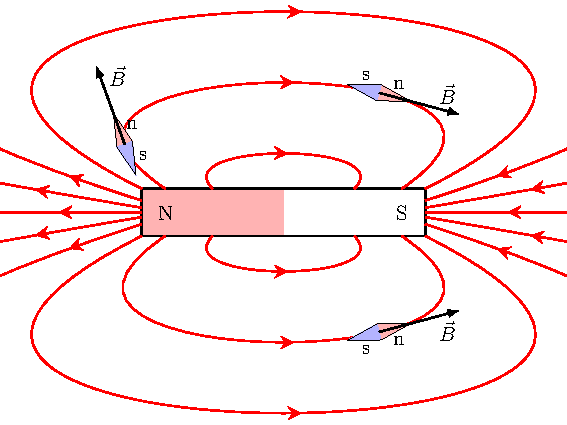
\includegraphics[width=\linewidth]{aim_ac}
		\label{fig:aim_ac}
	\end{center}
\end{minipage}

\subsubsection{Rails de \textsc{Laplace}}
\vspace{-20pt}
\noindent
\begin{minipage}[c]{.65\linewidth}
	Une autre manifestation remarquable est celle des \textbf{rails de
		\textsc{Laplace}}. Soit l'expérience représentée ci-contre~;
	on utilise un \textbf{aimant en U} pour créer un champ magnétique uniforme sur une assez
	grande partie d'un barreau métallique mobile, posé sur un bout de \textbf{circuit
		électrique}. Le \textbf{barreau} permet de \textbf{fermer le circuit}.
\end{minipage}
\hfill
\begin{minipage}[c]{.30\linewidth}
	\begin{center}
		\sswitch{
			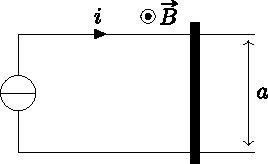
\includegraphics[width=\linewidth, draft=true]{rlp_1}
		}{
			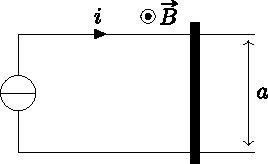
\includegraphics[width=\linewidth]{rlp_1}
		}
		\vspace{-15pt}
		\captionsetup{justification=centering}
		\captionof{figure}{\\Rails de \textsc{Laplace}.}
		\label{fig:rlp_1}
	\end{center}
\end{minipage}
\begin{tcn}(exem)<lftt>"obsv"{Observations}
	\begin{itemize}
		\item \psw{%
			      Lorsqu'on allume le courant, le barreau se met en mouvement \textbf{vers
				      la gauche}.
		      }%
		\item \psw{%
			      En inversant l'aimant \textbf{ou} en inversant le sens du courant, le
			      mouvement a lieu \textbf{dans l'autre sens}.
		      }%
		\item \psw{%
			      En mettant $\vv{B}$ dans le sens de la tige mobile, il n'y a pas de
			      mouvement.
		      }%
	\end{itemize}
\end{tcn}

Ces observations suggèrent l'existence d'une \textbf{force} dépendant du
\textbf{courant} et du \textbf{champ magnétique}, ainsi que de la
\textbf{direction} du barreau.

\subsection{Densité linéique de la force de \textsc{Laplace}}
\label{ssec:flplliq}

\begin{tcb*}(prop){Force de \textsc{Laplace} infinitésimale}
	Un élément de fil électrique de longueur $\dd{\ell}$ parcouru par un courant et
	plongé dans un champ magnétique $\Bf$ subit la force de \textsc{Laplace}~:
	\psw{%
		\[
			\boxed{\dd{\vv{F_{\textsc{Laplace}}}} = i \vv{\dd{\ell}}\wedge \vv{B}}
		\]
	}%
	avec $\vv{\dd{\ell}}$ orienté \textbf{dans le sens du courant}.
\end{tcb*}
On sait déjà qu'un \textbf{électron unique} en mouvement dans un champ subit la
force de \textbf{\textsc{Lorentz}}. Quand on s'intéresse à un grand ensemble
d'électrons, dans une \textbf{portion de conducteur}, celui-ci subit la force de
\textbf{\textsc{Laplace}}. Démontrons cette expression.

\begin{tcb*}(demo){Force infinitésimale de \textsc{Laplace}}
	\paragraph*{Hypothèses de calcul}~
	\begin{itemize}
		\item \psw{on suppose que les électrons sont animés d'une même vitesse
			      $\vv{v} = v \ux$, où $\ux$ désigne la direction du fil\footnote{Cette
				      hypothèse a pour but de simplifier le calcul~: dans la situation
				      réelle, $v$ représente la vitesse \textbf{moyenne} des électrons.}~;}
		\item \psw{le nombre d'électrons par unité de volume $n$ (en \si{m^{-3}})
			      est homogène~;}
		\item \psw{on considère un fil de section $S$ constante.}
	\end{itemize}

	\paragraph*{Expression de l'intensité du courant}~
	\smallbreak
	\noindent
	\begin{minipage}[c]{.65\linewidth}
		L'intensité représente le \textbf{flux de charge par seconde}. Pour la
		relier à notre fil, on doit s'intéresser à une \textbf{section imaginaire}
		et \textbf{compter le nombre d'électrons qui y passent} par seconde.
		\bigbreak
		\psw{%
			Pendant un intervalle $\dd{t}$, les électrons situés dans un cylindre de
			longueur $v \dd{t}$ en amont de $S$ vont passer à travers la section $S$~:
			$v \dd{t}$ correspond à la distance parcourue par les électrons pendant
			cet intervalle. Ceux qui sont plus loin ne la traversent pas. Dans ce
			cylindre, il y a $\dd{N} = n\times Sv \dd{t}$ électrons, soit une charge
			$\dd{q} = -e \dd{N} = -neSv \dd{t}$.
		}%
	\end{minipage}
	\hfill
	\begin{minipage}[c]{.30\linewidth}
		\begin{center}
			\sswitch{
				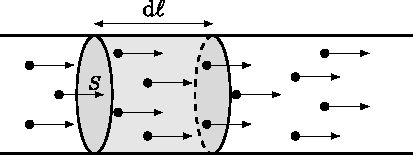
\includegraphics[width=\linewidth, draft=true]{cyl1}
			}{
				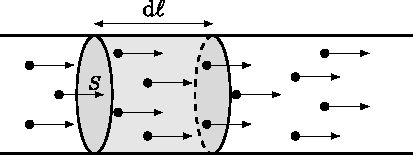
\includegraphics[width=\linewidth]{cyl1}
			}
			\vspace{-15pt}
			\captionof{figure}{Schéma fil.}
			\label{fig:cyl1}
		\end{center}
		D'où l'intensité du courant~:
		\setlength{\fboxsep}{3mm}
		\[
			\boxed{\psw{i = \dv{q}{t} = -neSv}}
		\]
	\end{minipage}

	\paragraph*{Expression de la force subie par une section de fil}~
	\smallbreak
	Considérons petit volume de longueur $\dd{\ell}$ de fil~:
	\smallbreak
	\begin{isd}[righthand ratio=.45]
		\begin{itemize}
			\setlength{\fboxsep}{3mm}
			\item Dans ce volume, il y a $\boxed{\psw{n\times S \dd{\ell}}}$ électrons.
			\item Chaque électron subit $\boxed{\psw{\vv{F\ind{\textsc{Lorentz}}} = -e
						      \vv{v} \wedge \vv{B}}}$.
		\end{itemize}
		\tcblower
		La force subie par la section de fil est donc
		\psw{%
			\begin{align*}
				\dd{\vv{F_{\textsc{Laplace}}}}         & = -neS \dd{\ell}\vv{v}\wedge \vv{B}
				\\\Lra
				\dd{\vv{F_{\textsc{Laplace}}}}         & = -neSv (\dd{\ell}\ux)\wedge \vv{B}
				\\\Lra
				\Aboxed{\dd{\vv{F_{\textsc{Laplace}}}} & = i \vv{\dd{\ell}}\wedge \vv{B}}
				\qed
			\end{align*}
		}%
	\end{isd}
\end{tcb*}

\subsection{Expression intégrale de la force de \textsc{Laplace}}
\label{ssec:lplint}
\begin{tcb*}(prop){Force de \textsc{Laplace}}
	La force de \textsc{Laplace} qui s'exerce sur une barre conductrice AC
	traversée par un courant $i$ et placée dans un champ magnétique
	\textbf{uniforme} et \textbf{stationnaire} $\vv{B}$ s'applique \textbf{en
		son milieu} et vaut~:
	\psw{%
		\[
			\boxed{\vv{F_{\textsc{Laplace}}} = i \vv{L}\wedge \vv{B}}
		\]
	}%
	où $i$ est orienté \textbf{selon le sens du vecteur} $\vv{L}$.
\end{tcb*}

\begin{tcb*}(demo){Force de \textsc{Laplace}}
	Si le champ magnétique est homogène sur un fil rectiligne AC, alors on
	\textbf{intègre} sur la longueur~:
	\smallbreak
	\begin{isd}
		\psw{%
			\begin{align*}
				\vv{F_{\textsc{Laplace}}}
				 & = \int_{\rm A}^{\rm B} i \vv{\dd{\ell}}\wedge \vv{B}
				\\\Lra
				\vv{F_{\textsc{Laplace}}}
				 & = i \left( \int_{\rm A}^{\rm C} \vv{\dd{\ell}}\right)\wedge \vv{B}
				\\\Lra
				\vv{F_{\textsc{Laplace}}}
				 & = i \vv{L}\wedge \vv{B}
				\qed
			\end{align*}
			Avec $\int_{\rm A}^{\rm C} \vv{\dd{\ell}} = \vvr{AC} = \vv{L}$
		}%
		\tcblower
		\begin{center}
			\sswitch{
				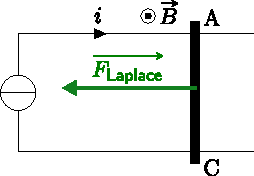
\includegraphics[scale=1, draft=true]{rlp_2}
			}{
				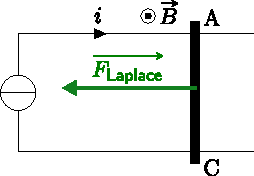
\includegraphics[scale=1]{rlp_2}
			}
			\captionof{figure}{Schéma rails.}
			\label{fig:rlp_2}
		\end{center}
	\end{isd}
\end{tcb*}

\begin{tcb}(rema)<lftt>'l'{Force de \textsc{Laplace}}
	\begin{minipage}[t]{.68\linewidth}
		\begin{enumerate}
			\item On peut orienter la force selon la règle de la main droite, version
			      «~trois doigts~»~:
			      \begin{itemize}
				      \item \psw{%
					            la force sur le pouce («~le pouce pousse~»)~;
				            }%
				      \item \psw{%
					            l'\textbf{in}tensité sur l'\textbf{in}dex~;
				            }%
				      \item \psw{%
					            le champ \textbf{ma}gnétique sur le \textbf{ma}jeur.
				            }%
			      \end{itemize}
			\item Cette expression permet d'obtenir la dimension de $B$ en fonction des
			      dimensions fondamentales~:
			      \psw{%
				      \[
					      B = \frac{F}{\ell i} \Lra [B]
					      = \frac{\rm M \cdot L \cdot T^{-2}}{\rm L \cdot I}
					      = \mathrm{M \cdot T^{-2} \cdot I^{-1}}
				      \]
			      }%
		\end{enumerate}
	\end{minipage}
	\hfill
	\begin{minipage}[t]{.30\linewidth}
		~
		\vspace*{-20pt}
		\begin{center}
			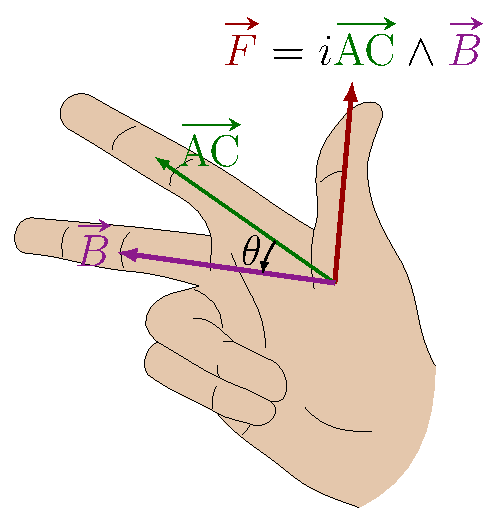
\includegraphics[width=\linewidth]{righthand_laplace}
			\label{fig:ra_lpl}
		\end{center}
	\end{minipage}
	\begin{enumerate}[start=3]
		\item L'ordre de grandeur de cette force pour un fil de \SI{5}{cm} dans un
		      champ de \SI{0.1}{T} parcouru par une intensité de \SI{1}{A} est~:
		      \psw{%
			      \[
				      \boxed{\norm{\vv{F_{\textsc{Laplace}}}} = i \ell B = \SI{5}{mN}}
			      \]
		      }%
		      \vspace{-15pt}
	\end{enumerate}
\end{tcb}

\begin{tcb*}[sidebyside](impl){Puissance de la force de \textsc{Laplace}}
	La puissance de la force de \textsc{Laplace} correspondante est~:
	\psw{%
		\[
			\boxed{
				\Pc_{L,v}
				= \left( i \vv{L}\wedge \vv{B} \right) \cdot \vv{v}}
		\]
	}%
	\tcblower
	Ainsi, alors que la force de magnétique de \textsc{Lorentz} était de
	puissance nulle sur \textbf{1 électron}, ça n'est pas le cas de la force
	de \textsc{Laplace} qui s'applique sur un solide conducteur~: dans ce
	cas, \textbf{un champ magnétique peut accélérer le système}.
\end{tcb*}

\section{Le couple des actions de \textsc{Laplace}}
\label{sec:lplcpl}

\subsection{Spire rectangulaire plongée dans un champ constant}
\label{ssec:lplcplspire}

\begin{tcb*}(prop){Couple de \textsc{Laplace}}
	Un \textbf{circuit ou un aimant} de moment magnétique $\vv{\mu}$ plongé dans
	un champ \textbf{uniforme} et \textbf{stationnaire} $\vv{B}$ subit un
	\textbf{couple magnétique}, issu du moment des forces de \textsc{Laplace} par
	rapport à un axe $\uz$ tel que~:
	\psw{%%
		\[
			\boxed{\Gf_{\mathrm{Lap}} = \vv{\mu}\wedge \Bf}
		\]
	}%
	\vspace{-15pt}
\end{tcb*}
On commence par un cas particulier~: une spire rectangulaire dans un champ
constant. Vérifions l'expression.
\begin{tcb*}[breakable](demo){Couple de \textsc{Laplace}}
	\paragraph*{Modélisation}
	\begin{itemize}
		\item On considère un cadre rectangulaire AECD parcouru par un courant $i$. Ce
		      cadre peut tourner autour de l'axe $(\Or z)$.
		\item On impose un champ magnétique uniforme $\vv{B} = B\ux$. On note $\th$
		      l'angle entre $\vv{B}$ et la normale au cadre, orientée \textbf{dans le sens
			      de} $i$. On note cette normale $\vv{n}$.
	\end{itemize}
	\begin{isd}[lefthand ratio=.35]
		\begin{center}
			\includegraphics[height=5.5cm]{spir2_clip}
			\captionof{figure}{Schéma simple.}
			\label{fig:spir1_a}
		\end{center}
		\tcblower
		\begin{center}
			\sswitch{
				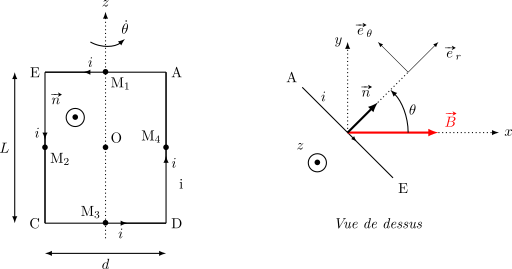
\includegraphics[scale=.8, draft=true]{spir1}
			}{
				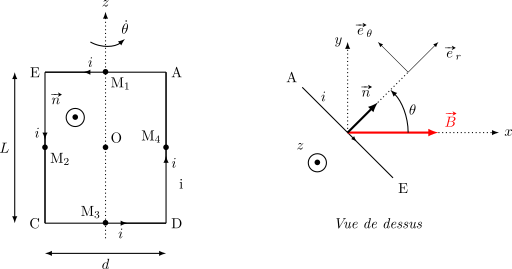
\includegraphics[scale=.8]{spir1}
			}
			\vspace{-15pt}
			\captionof{figure}{Schéma étendu.}
			\label{fig:spir1_b}
		\end{center}
	\end{isd}
	\paragraph*{Résultante des forces}~
	\smallbreak
	Il s'agit d'additionner les différentes forces de \textsc{Laplace} subies par
	chacun des côtés de la spire rectangulaire\ftn{Tant que le champ magnétique
		est homogène, alors peu importe le circuit fermé, on aura $\DS
			\oint_{\mathcal{C}}^{} i \vv{\dd{\ell }}\wedge \vv{B} =
			i \left( \oint_{\mathcal{C}} \vv{\dd{\ell }} \right)\wedge \vv{B} =
			\vv{0}$ }~:
	%   Sur le côté AE par exemple~:
	% \[
	% 	\vv{F_{\textsc{Lap}, \rm AE}} = i \vv{\rm AE}\wedge \vv{B}
	% \]
	% La résultante est donc
	% \begin{align*}
	% 	\sum \vv{F\ind{Lap}} & =
	% 	\psw{%
	% 		i \vv{\rm AE}\wedge \vv{B} +
	% 		i \vv{\rm EC}\wedge \vv{B} +
	% 		i \vv{\rm CD}\wedge \vv{B} +
	% 		i \vv{\rm DA}\wedge \vv{B}
	% 	}%
	% 	\\\Lra
	% 	\sum \vv{F\ind{Lap}} & =
	% 	\psw{%
	% 		i
	% 		\big( \underbracket[1pt]{\vv{\rm AE} + \vv{\rm EC} + \vv{\rm CD} + \vv{\rm DA}}_{=\of} \big)
	% 		\wedge
	% 		\vv{B}
	% 	}%
	% 	\\\Lra
	% 	\sum \vv{F\ind{Lap}} & = \psw{\vv{0}}
	% \end{align*}
	\begin{gather*}
		\sum \vv{F\ind{Lap}} =
		\psw{%
			i \vvr{AE}\wedge \vv{B} +
			i \vvr{EC}\wedge \vv{B} +
			i \vvr{CD}\wedge \vv{B} +
			i \vvr{DA}\wedge \vv{B}
			=
			i
			\big( \underbracket[1pt]{\vv{\rm AE} + \vv{\rm EC} + \vv{\rm CD} + \vv{\rm DA}}_{=\of} \big)
			\wedge
			\vv{B}
			= \of
		}%
	\end{gather*}
	% \begin{center}
	% 	\begin{tcb}[width=.8\linewidth](rema)<lft>'l'{Remarque}
	% 		Tant que le champ magnétique est homogène, alors peu importe le circuit fermé,
	% 		on aura
	% 		\psw{%
	% 			\[
	% 				\oint_{\mathcal{C}}^{} i \vv{\dd{\ell }}\wedge \vv{B} =
	% 				i \left( \oint_{\mathcal{C}} \vv{\dd{\ell }} \right)\wedge \vv{B} = \vv{0}
	% 			\]
	% 		}%
	% 		\vspace{-15pt}
	% 	\end{tcb}
	% \end{center}
	\paragraph*{Moment des forces}
	\begin{itemize}
		\item[b]{AE}:~
		\smallbreak
		\vspace{-25pt}
		\begin{isd}[interior hidden, sidebyside align=top]
			\tcbsubtitle{\fatbox{\textbf{Force}}}
			\begin{align*}
				\vv{F\ind{Lap,AE}}
				 & =
				\psw{i \vv{\rm AE}\wedge \vv{B}}
				\\
				 & = \psw{i (-d \cos{\th}\uy + d\sin{\th}\ux)\wedge \vv{B}}
				\\
				 & = \psw{idB\cos{\th}\uz}
			\end{align*}
			\tcblower
			\tcbsubtitle{\fatbox{\textbf{Moment}}}
			% La force s'exerce de façon constante tout le long de la spire, donc son point
			% d'application est $\Mr_1$, qui est un point de l'axe de rotation. Ainsi,
			% \textbf{son moment est nul}~:
			Elle s'applique en $\Mr_1 \in (\Or z)$, soit
			\[
				\psw{%
					\boxed{\Mcf\ind{O} \left( \vv{F\ind{Lap,AE}} \right) =
						\vvr{OM_1}\wedge \vv{F\ind{Lap,AE}}
						= \of}
				}%
			\]
		\end{isd}
		\item[b]{EC}:~
		\smallbreak
		\vspace{-25pt}
		\begin{isd}[interior hidden, sidebyside align=top, lefthand ratio=.3]
			\tcbsubtitle{\fatbox{\textbf{Force}}}
			\begin{align*}
				\vv{F\ind{Lap,EC}}
				 & = \psw{i \vv{\rm EC}\wedge \vv{B}}
				\\
				 & = \psw{i (-L\uz)\wedge B\ux}
				\\
				 & = \psw{-iLB\uy}
			\end{align*}
			\tcblower
			\tcbsubtitle{\fatbox{\textbf{Moment}}}
			% La force s'exerce de façon constante tout le long de la spire, donc son point
			% d'application est $\Mr_1$, qui est un point de l'axe de rotation. Ainsi,
			% \textbf{son moment est nul}~:
			Elle s'applique en $\Mr_2$, soit
			\begin{align*}
				\Mcf\ind{O} \left( \vv{F\ind{Lap,EC}} \right)
				 & = \psw{\vvr{OM_2}\wedge \vv{F\ind{Lap,EC}}}
				\\
				 & =
				\psw{%
					\left(
					-\frac{d}{2}\cos{\th}\uy +
					\frac{d}{2}\sin{\th}\ux
					\right)\wedge -iLB\uy
				}%
				\\\Lra
				\Mcf\ind{O} \left( \vv{F\ind{Lap,EC}} \right)
				 & = \psw{-iLB \frac{d}{2}\sin{\th}\uz}
			\end{align*}
		\end{isd}
		\item[b]{CD}:~
		La force agissant sur le côté $\vvr{CD}$ s'applique en $\Mr_3$, qui est sur
		l'axe de rotation, donc immédiatement~:
		\psw{%
			\[
				\boxed{\Mcf\ind{O} \left( \vv{F\ind{Lap,CD}} \right) = \of}
			\]
		}%
		\item[b]{DA}:~
		De manière analogue au côté $\vvr{EC}$ (on vérifie avec la règle de la
		main droite)~:
		\smallbreak
		\vspace{-15pt}
		\begin{isd}[interior hidden, sidebyside align=top]
			\tcbsubtitle{\fatbox{\textbf{Force}}}
			\psw{%
				\[
					\vv{F\ind{Lap,DA}} = iLB\uy
				\]
			}%
			\tcblower
			\tcbsubtitle{\fatbox{\textbf{Moment}}}
			Elle s'applique en $\Mr_4$, soit
			\psw{%
				\begin{gather*}
					\boxed{\Mcf\ind{O} \left( \vv{F\ind{Lap,DA}} \right)
						= -iLB \frac{d}{2}\sin{\th}\uz}
				\end{gather*}
			}%
		\end{isd}
		% Et enfin sur le côté $\vv{\rm DA}$~:
		% \begin{hide}
		% \begin{align*}
		% 	\vv{F\ind{Lap,DA}}
		% 	 & = i \vv{\rm DA}\wedge \vv{B}
		% 	\\
		% 	 & = i (L\uz)\wedge B\ux
		% 	\\
		% 	 & = iLB\uy
		% \end{align*}
		% 	Le point d'application est $\Mr_4$, donc~:
		% 	\begin{align*}
		% 		\Mc_z \left( \vv{F\ind{Lap,DA}} \right)
		% 		 & = \left( \vv{\rm OM_4} \wedge \vv{F\ind{Lap,DA}} \right)\cdot \uz
		% 		\\
		% 		 & = \left(
		% 		\left(
		% 			\frac{d}{2}\cos{\th}\uy
		% 			- \frac{d}{2}\sin{\th}\ux
		% 			\right)\wedge iLB\uy
		% 		\right)\cdot \uz
		% 		\\\Lra
		% 		\Aboxed{\Mc_z \left( \vv{F\ind{Lap,DA}} \right)
		% 		 & = -iLB \frac{d}{2}\sin{\th}}
		% 	\end{align*}
		% \end{hide}
		% \noindent
	\end{itemize}
	\vspace{-30pt}
	\paragraph*{Couple des forces}~
	\smallbreak
	\begin{isd}
		En sommant tous ces moments, on trouve donc~:
		\psw{%
			\begin{align*}
				\Gf\ind{Lap}         & =
				\sum_i \Mcf\ind{O}\left( \vv{F_{\mathrm{Lap},i}} \right)
				\\\Lra
				\Aboxed{\Gf\ind{Lap} & = -idLB\sin{\th} \uz}
			\end{align*}
		}%
		\vspace{-15pt}
		\tcblower
		Avec le moment magnétique de la spire $\vv{\mu} = iS \vv{n}$, on trouve~:
		\psw{%
			\begin{align*}
				\vv{\mu}\wedge \vv{B}
				 & = iS (\cos{\th}\ux+\sin{\th}\uy \wedge B\ux)
				\\
				 & = -iSB\sin{\th}\uz
				\\
				 & = -iLdB\sin{\th}\uz
				\qed
			\end{align*}
		}%
		\vspace{-15pt}
	\end{isd}
\end{tcb*}

\begin{tcb*}[sidebyside](impl){Puissance du couple de \textsc{Laplace}}
	La puissance du couple de \textsc{Laplace} correspondante est~:
	\psw{%
		\[
			\boxed{
				\Pc_{L,\w}
				= \Gf_{L} \cdot \wf
			}
		\]
	}%
	avec $\wf$ la vitesse angulaire de rotation.
	\tcblower
	Pour un circuit de vitesse de translation $\vf$ et de vitesse angulaire $\wf$,
	on aura
	\psw{%
		\[
			\boxed{\Pc_L = \Ff_L \cdot \vf + \Gf_L \cdot \wf}
		\]
	}%
\end{tcb*}

\subsection{Effet sur un aimant}
\label{ssec:lplcplaim}

Par analogie avec la spire, on peut dire qu'un moment magnétique soumis à un
champ magnétique génère un couple de forces, de couple résultant~:
\smallbreak
\noindent
\begin{minipage}[t]{.5\linewidth}
	\[
		\Gf_L =  \vv{m}\wedge \vv{B}
	\]
\end{minipage}
\hfill
\begin{minipage}[t]{.5\linewidth}
	~
	\vspace*{-30pt}
	\begin{center}
		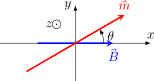
\includegraphics[scale=1]{aim_cpl}
		\label{fig:aim_cpl}
	\end{center}
\end{minipage}

\begin{tcb*}[breakable](appl)<lftt>'l'{Oscillations d'un aimant}
	\begin{enumerate}
		\item Exprimer le couple de \textsc{Laplace} subit par $\vv{m}$ en fonction
		      de $\th$.
		\item En déduire les positions d'équilibre de $\vv{m}$.
		\item En étudiant dans quel sens le couple de \textsc{Laplace} tend à faire
		      tourner $\vv{m}$ en cas de petites perturbations, déterminer la
		      stabilité des deux positions d'équilibre.
	\end{enumerate}
	\tcblower
	\begin{enumerate}
		\item \psw{%
			      On a
			      \begin{align*}
				      \vv{m} & = m \left( \cos{\th}\ux + \sin{\th}\uy \right)
				      \\
				      \text{et} \quad
				      \vv{B} & = B_0\ux
			      \end{align*}
			      D'où
			      \[
				      \boxed{\Gf = -mB_0\sin{\th}\uz}
			      \]
			      Ce qui fait tourner le système autour de l'axe $z$.
		      }%
		\item \psw{%
			      On est à l'équilibre si la somme des forces et la somme des
			      moments sont nulles. Avec uniquement le couple magnétique, on a
			      bien une résultante nulle~: on a donc équilibre si $\Gf = \vv{0}$,
			      soit
			      \begin{gather*}
				      \sin{\th\ind{eq}} = 0
				      \Lra
				      \left\{
				      \begin{array}{rl}
					      \th\ind{eq} & = 0 \quad \text{ou}
					      \\
					      \th\ind{eq} & = \pi
				      \end{array}
				      \right.
			      \end{gather*}
		      }%
		\item
		      \begin{itemize}
			      \item \psw{%
				            En $\th\ind{eq} = \pi$, une petite déviation vers le haut
				            donne un mouvement de rotation dans le sens horaire, qui
				            écarte donc l'aimant de sa position d'équilibre~: il est
				            \textbf{instable}.
			            }%
			      \item
			            \psw{%
				            À l'inverse, en $\th\ind{eq} = 0$, une petite
				            déviation vers le haut donne un mouvement de rotation dans
				            le sens direct, le ramenant à sa position d'équilibre~: il
				            est \textbf{stable}.
			            }%
		      \end{itemize}
	\end{enumerate}
\end{tcb*}

La dynamique de la rotation de l'aimant est alors équivalente à celle du pendule
pesant~! En effet, en appliquant le théorème du moment cinétique à l'aimant~:
\psw{%
	\[
		\dv{\Lc_z}{t} = J\tpp = \sum \Mc_z
	\]
}%
avec $J$ le moment d'inertie par rapport à l'axe de rotation. Or,
d'après ce qui précède,
\psw{%
	\begin{align*}
		\sum \Mc_z                           & = -mB\sin{\th}
		\\\Lra
		J\tpp                                & = -mB\sin{\th}
		\\\Lra
		\Aboxed{\tpp + \frac{mB}{J}\sin{\th} & = 0}
	\end{align*}
}%
qui est bien l'équation du pendule.
\begin{tcb*}(ror){Action d'un champ sur un aimant}
	\psw{%
		Du fait des petites vibrations (qui rendent la position $\th=\pi$ non
		durable) et des frottements qui arrêtent sa course, \textbf{un aimant tend à
			s'aligner sur le champ magnétique}, et ce d'autant plus vite que le champ
		$\vv{B}$ est intense.
	}%
\end{tcb*}
En effet, au voisinage de
la position d'équilibre, on a $\sin{\th} \sim \th$, d'où
\psw{%
	\[
		\tpp + \frac{mB}{J}\th = 0
	\]
}%
qui est l'équation d'un \textbf{oscillateur harmonique}, de période propre~:
\psw{%
	\[
		T_0 = 2\pi \sqrt{\frac{J}{mB}}
	\]
}%

\subsection{Boussole sur Terre}
\label{ssec:boussoleterre}
\vspace{-15pt}
\noindent
\begin{minipage}[c]{.64\linewidth}
	On peut donc pleinement expliquer l'alignement d'une boussole à la surface de la
	Terre, toujours en modélisant son champ magnétique par un aimant~: l'aiguille
	aimantée de moment magnétique $\vv{\mu}$ s'oriente spontanément sur le champ
	magnétique terrestre.
	\bigbreak
	On notera bien que dans ce cas, la boussole pointe bien vers le Nord
	géographique, mais qu'il correspond au pôle Sud magnétique de l'aimant par
	lequel on représente la Terre\ftn{Le Nord magnétique reste au Nord~! On parle
		ici du pôle sud \textbf{de l'aimant}.}.
\end{minipage}
\hfill
\begin{minipage}[c]{.35\linewidth}
	\begin{center}
		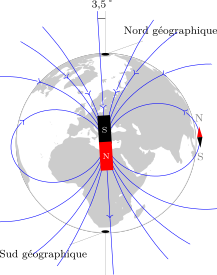
\includegraphics[scale=.7]{boussole_terre}
		\label{fig:bterre}
	\end{center}
\end{minipage}

\subsection{Effet moteur d'un champ magnétique tournant}
\label{ssec:btourne}
Si un aimant a tendance à s'orienter sur un champ magnétique, on peut utiliser
ce couple pour forcer la rotation continue d'un aimant grâce à un \textbf{champ
	tournant}~: c'est le principe du \textbf{moteur synchrone}.
\begin{tcb}(defi){Champ magnétique tournant}
	\begin{minipage}[c]{.6\linewidth}
		Un champ tournant est un champ de \textbf{norme constante}, mais dont la
		\textbf{direction tourne} à vitesse angulaire constante.
		\smallbreak
		Par le couple de \textsc{Laplace}, un \textbf{aimant} soumis à ce champ tournera en
		régime stationnaire à la \textbf{même vitesse} angulaire $\w$.
	\end{minipage}
	\hfill
	\begin{minipage}[c]{.4\linewidth}
		~
		\begin{center}
			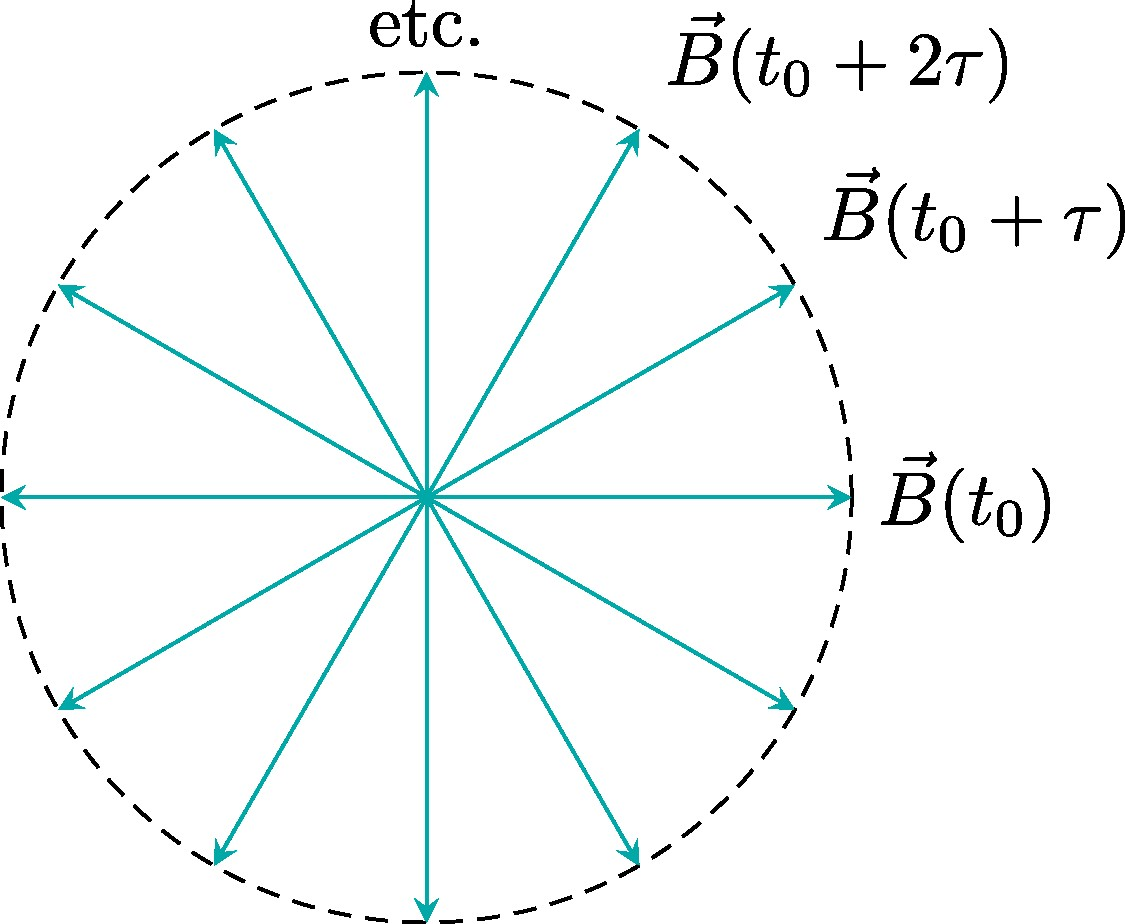
\includegraphics[scale=.9]{btourn1}
			\captionsetup{justification=centering}
			\captionof{figure}{\\Champ magnétique tournant.}
			\label{fig:btourn1}
		\end{center}
	\end{minipage}
\end{tcb}
\noindent
\begin{minipage}[t]{.64\linewidth}
	Pour réaliser un champ tournant, on peut utiliser deux bobines identiques, de
	courants déphasés de $\pi/2$~:
	\begin{align*}
		i_1(t) & = \psw{I_0\cos{\wt}}
		\\\qqet
		i_2(t) & = \psw{I_0\cos{\wt-\pi/2} = I_0\sin{\wt}}
	\end{align*}
	Ainsi, proche de l'axe des bobines on aura des champs
	\begin{gather*}
		\vv{B_1}(t) = \psw{k I_0\cos{\wt}\,\ux}
		\qqet
		\vv{B_2}(t) = \psw{k I_0\sin{\wt}\,\uy}
	\end{gather*}
	Soit, par somme~:
	\psw{%
		\[
			\boxed{\vv{B} = k I_0 (\cos{\wt}\ux + \sin{\wt}\uy) = k I_0\ur}
		\]
	}%
	qui est bien un champ tournant.
\end{minipage}
\hfill
\begin{minipage}[t]{.35\linewidth}
	~
	\begin{center}
		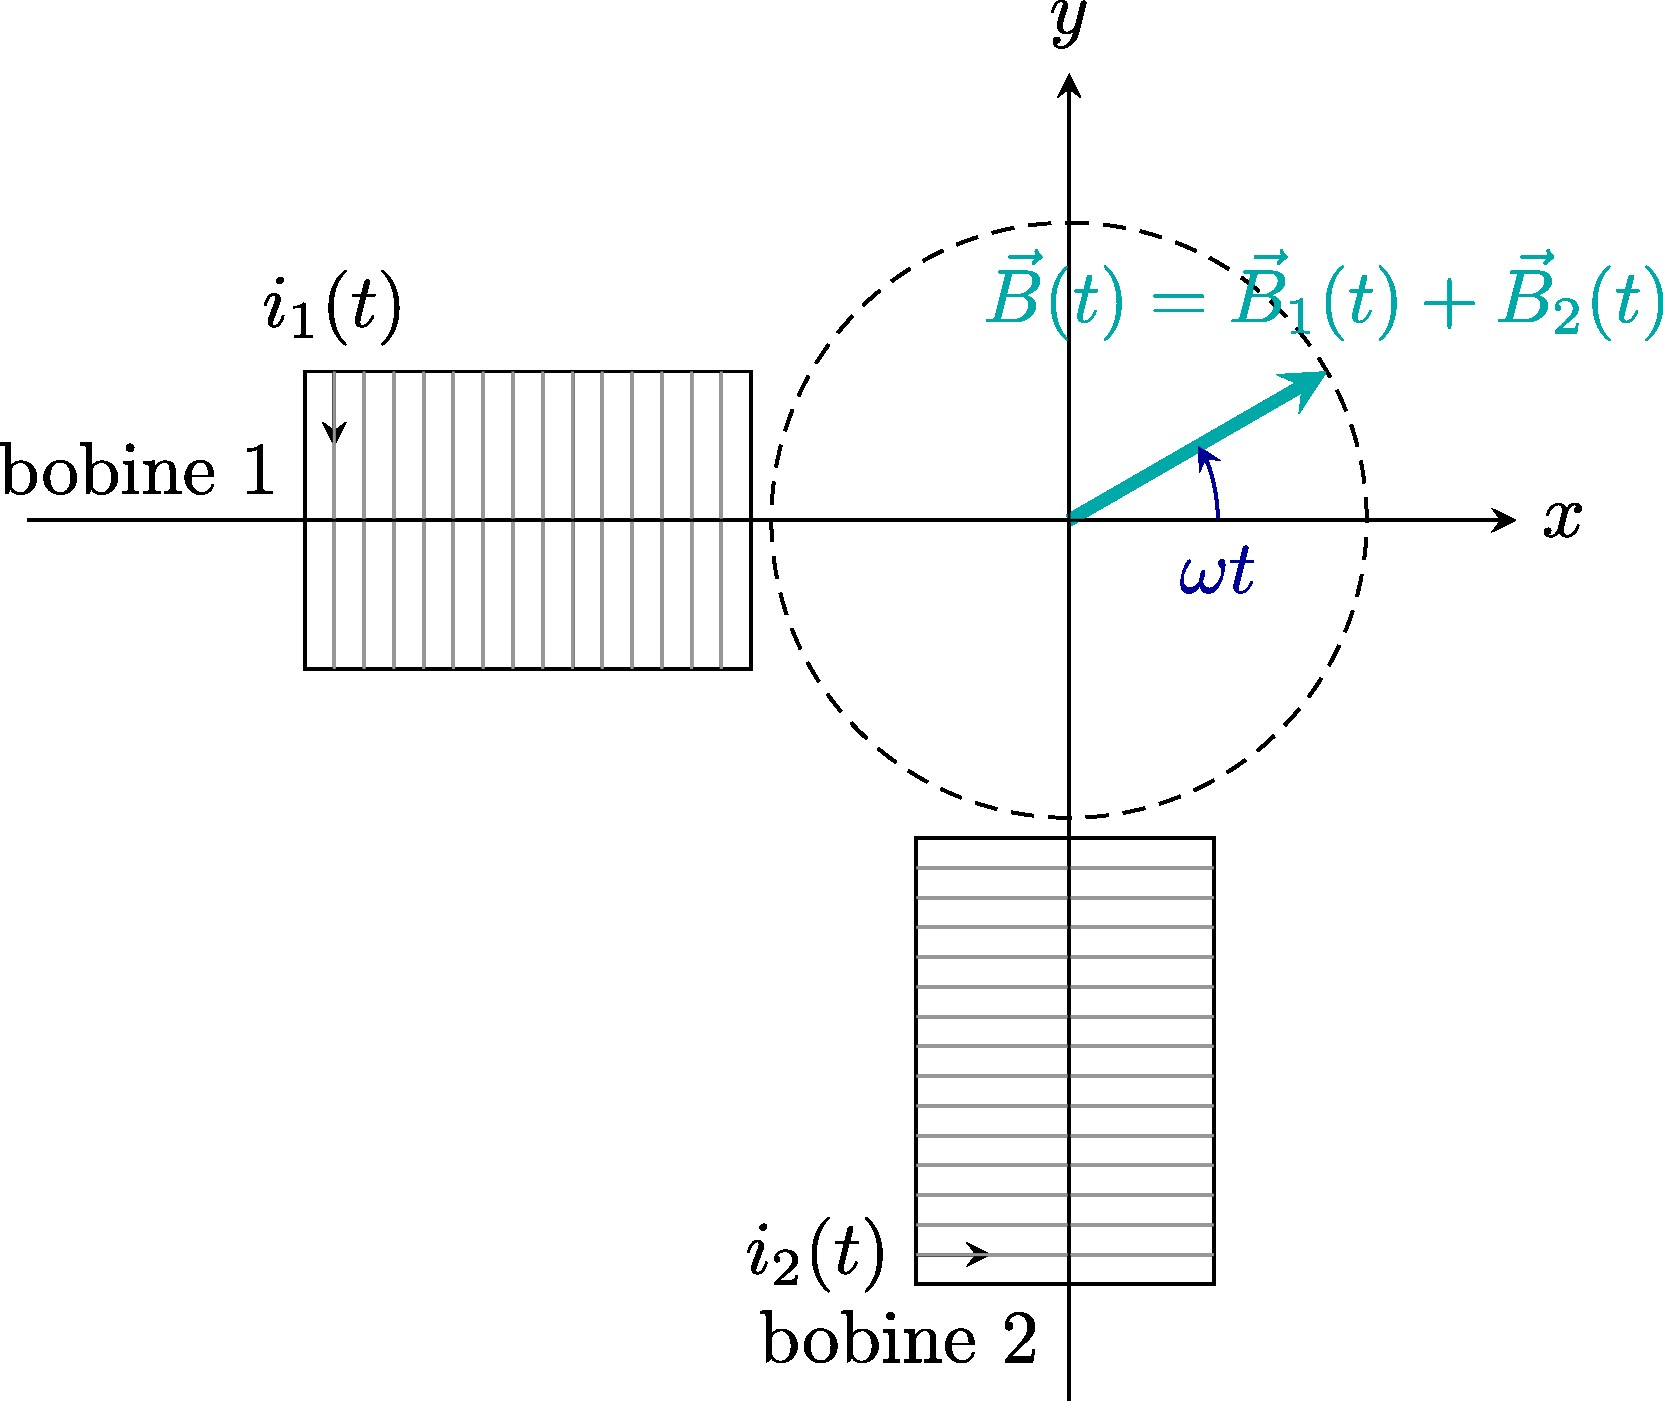
\includegraphics[scale=1]{btourn2}
		\label{fig:btourn2}
	\end{center}
\end{minipage}
Il est également possible de faire un champ tournant à l'aide de trois bobines,
décalées de $2\pi/3$~: c'est ce qu'on appelle un courant \textbf{triphasé}, et
c'est ce qui est utilisé dans le transport d'électricité de manière
industrielle.

\end{document}
